\chapter{Построение решений задач}
\label{sec:Chapter3} \index{Chapter3}

После анализа литературы и уже существующих решений стало ясно, как реализовывать каждую из поставленных ранее задач. Далее будет рассказано о том, какие методы были выбраны для выполнения этих задач. Порядок, в котором они были объявлены в главе \ref{sec:Chapter1} сохранен.

\section{Признаки для датасета}

Обсудим признаки, которые были выбраны для обучения классификатора. В предыдущей главе \ref{sec:Chapter2} было сказано, что из всех признаков, указанных в \cite{HECKMAN2011363}, данная работа сфокусируется лишь на первых двух - характеристики ошибки и характеристики кода, опуская последние три - метрики репозитория с исходным кодом, метрики базы данных с багами, метрики динамического анализа. Далее будет описано, почему при составлении датасета был опущен каждый из перечисленных классов признаков, а также будет описано то, какие признаки все же были представлены в датасете в настоящей работе.

\subsection{Метрики репозитория с исходным кодом}
Как было обозначено в обзоре литературы \ref{sec:Chapter2}, для того, чтобы хоть сколько нибудь эффективно анализировать историю коммитов проекта, она должна быть строго организована, иначе поиск нужных мест в коде сводится к полному анализу всего проекта на каждом из этапов его разработки. В той же главе было объяснено, что в открытом доступе очень малое число проектов соблюдает подобные правила. Плюс, даже при их соблюдении, множественный анализ проекта очень дорог вычислительно и по времени. Плюс, для того, чтобы размечать false positives, необходимо иметь доступ к уже собранной статистике использования анализатора, которой не существует в открытом доступе. Таким образом, анализ истории коммитов и других метрик репозитория отпадает.

\subsection{Метрики базы данных с багами}
Как и в предыдущем пункте, применение данных метрик ограничивается их отсутствием в открытом доступе.

\subsection{Метрики динамического анализа}
Для проведения динамического анализа требуется полная сборка всего проекта, что добавляет сложности к и без того затратному процессу анализа. Также, основным предметом изучения данной работы является именно статический анализ, поэтому рассмотрение метрик динамического анализа было решено оставить как предмет для будущих исследований.

\subsection{Характеристики ошибки}
\label{sec:Err-to-CWE} \index{Err-to-CWE}
Для того, чтобы удовлетворить требованию языковой независимости, все сообщения анализаторов требуется приводить к общему виду. Таким общим видом было выбрано представление Common Weakness Enumeration (CWE)\cite{CWE-doc}. Таким образом, добавление нового статического анализатора к списку поддерживаемых сводится к добавлению интерфейса, транслирующего код ошибки анализатора в код CWE. К счастью, для большинства распространенных статических анализаторов существуют таблицы соответствия или настройки, позволяющие выводить код ошибки сразу в формате CWE.

\subsection{Характеристики кода}
В проанализированной литературе основными признаками, по которым производилось обучение, являлись метрики кода. Чаще всего речь шла о метриках таких как вложенность, цикломатическая сложность, количество путей через выделенный фрагмент кода, etc. В данной работе метрики кода считались только для функции, в которой анализатор обнаружил уязвимость. Замеры производились при помощи утилиты ccsm\cite{CCSM}, в которую были дополнительно внесены изменения. Реализована данная утилита как инструмент в инфраструктуре Clang\cite{Clang}. Этот инструмент вызывает парсер Clang для указанного файла, и работает с полученным частичным промежуточным представлением. Т.к. полная компиляция проекта не требуется (парсинг производится лишь на выбранном файле), то извлечение этих метрик не сказывается на общем времени сбора датасета. Метрики кода, использованные для обучения моделей в данной работе можно разделить на следующие группы:

\begin{enumerate}
    \item Количество ключевых слов, контролирующих поток исполнения программы (for, if, else, etc.)
    \item Различные способы подсчета цикломатической сложности
    \item Количество различных обращений к памяти (разименование указателя, обращение к полю, обращение к полю по указателю, etc.)
    \item Характеристики самой функции (количество путей через нее, вложенность)
\end{enumerate}

\subsection{Token-based представление кода}
\label{sec:Tokens} \index{Tokens}
Описанные выше метрики характеризуют код лишь косвенно, не давая представления о его структуре. Таким образом теряется способность классификатора распознавать шаблоны, которые приводят к false positive. Чтобы бороться с этой проблемой был предложен подход на основе токенов. Токены были выбраны, т.к. анализ AST является затруднительным и более затратным. Токены, с другой стороны, можно получить еще на этапе лексического анализа. Вывод токенов был также реализован в качестве инструмента для Clang. Чтобы увеличить шансы на распознавание шаблонов false positive, представление кода в виде токенов было предварительно обработано: были оставлены только ключевые слова, влияющие на поток исполнения, операторы и идентификаторы.

\begin{figure}[H]
    \centering
    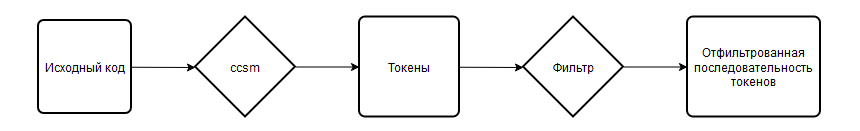
\includegraphics[width=\textwidth]{flow.png}
    \caption{Шаги получения отфильтрованной последовательности токенов}
\end{figure}

После предварительной обработки, из получившейся последовательности токенов выбирается подпоследовательность фиксированной длины, такая, что токен, на который указывает сообщение об ошибке находится ровно посередине подпоследовательности. Получившаяся подпоследовательность фиксированной длины называется окном и контролируется гиперпараметром WINDOW\_SIZE, отвечающим за ширину этого окна. Соответственно, в датасете появляются признаки token[0], token[1], token[2], ... token[WINDOW\_SIZE - 1]. Предположение данной работы состоит в том, что последовательности отфильтрованных токенов наряду с метаданными о коде должно хватить для распознавания большинства шаблонов false positive, указанных в \cite{Reynolds}.
\\
\\
Резюмируя, датасет, используемый для обучения моделей в данной работе, имеет следующий вид:

\begin{table}[H]
    \centering
    \resizebox{\textwidth}{!}{
        \begin{tabular}{|c|c|c|c|c|c||c|}
            \hline
            код CWE & token[0] & token[1] & ... & token[WINDOW\_SIZE - 1] & метрики кода & метка класса \\ \hline
        \end{tabular}
    }
    \caption{Общий вид элемента датасета}
\end{table}

\section{Метод генерации и разметки датасета}
Для генерации и разметки датасета была выбрана кодовая база Juliet Test Suite\cite{Juliet}. Имеющиеся в коде метаданные позволяют без проблем классифицировать большинство сообщений анализатора как false positive или true positive. Рассмотрим пример кода Juliet Test Suite:

\begin{verbatim}
    // CWE415_Double_Free__malloc_free_char_08.c
    ...
    void CWE415_Double_Free__malloc_free_char_08_bad()
    {
        char * data;
        /* Initialize data */
        data = NULL;
        if(staticReturnsTrue())
        {
            data = (char *)malloc(100*sizeof(char));
            if (data == NULL) {exit(-1);}
            /* POTENTIAL FLAW: Free data in the source - the bad sink frees data as well */
            free(data);
        }
        if(staticReturnsTrue())
        {
            /* POTENTIAL FLAW: Possibly freeing memory twice */
            free(data);
        }
    }
    ...

    // manifest.xml
    ...
    <testcase>
      <file path="CWE415_Double_Free__malloc_free_char_08.c">
        <flaw line="47" name="CWE-415: Double Free"/>
      </file>
    </testcase>
    ...
\end{verbatim}

Juliet Test Suite содержит два типа метаданных, которые полезны при оценке верности предупреждений анализатора:
\begin{enumerate}
    \item manifest.xml - этот файл содержит точную информацию о каждой ошибке, включая номер строки, файл и тип ошибки.
    \item Названия функций - в документации к тестовой сюите говорится, что если название функции содержит строку 'GOOD', то указанный тип CWE в данной функции не встречается, а если название функции содержит строку 'BAD', то данный CWE в этой функции присутствует.
\end{enumerate}

Для разметки датасета были собраны следующие данные: для каждого файла, в котором анализаторы находили уязвимости были собраны метрики кода, а также token-based представление для каждой из функций. Далее стоит учитывать, что Juliet Test Suite указывает только на наличие или отсутствие конкретного CWE, указанного в названии файла, тоесть мы не можем выносить суждение о других типах уязвимостей, о которых сообщил анализатор в данном файле. Иными словами, если уязвимость, найденная анализатором не совпадает с CWE, указанным в manifest.xml или названии файла, то метаданные не могут быть использованы для того, чтобы пометить данное сообщение анализатора как true positive / false positive. Таким образом, после того, как вся тестовая сюита была проанализирована несколькими анализаторами, их сообщения об уязвимостях были слиты в единую базу данных, где каждый код ошибки был предварительно заменен на эквивалентный CWE либо при помощи встроенных в анализатор средств, либо при помощи уже заранее составленных таблиц соответствия. Далее, для каждого сообщения об ошибке была получена метка класса. Разметка происходила следующим образом:

\begin{enumerate}
    \item Если информация об уязвимости в manifest.xml (путь, строка, тип) совпадает с той, которую сообщил анализатор, то ставилась метка true positive
    \item Если уязвимость обнаружена в строках, принадлежащих функции с именем 'GOOD', и код ошибки совпадает с CWE, указанным в имени файла, то ставилась метка false positive.
\end{enumerate}

Для остальных случаев невозможно точно определить метку. Однако существуют спекулятивные методы, которые являются предметом для дальнейших исследований и не были рассмотрены в данной работе. Их применение позволит расширить кодовую базу, на которой обучается классификатор, что увеличит качество и количество распознаваемых шаблонов false positive.

\section{Обучение классификатора}



\subsection{Decision tree}
\subsection{Gradient boosting}


\newpage